\chapter{System results}\label{chap:sysres}

\label{sec:sysRes}
The complete circuit charging characteristics are documented in table \ref{tab:batsys}. The current measurements are calculated from the TSC output using eq.\ref{eq:refeq}. A2 output refers to the output of the second assignment which can be seen in figure \ref{fig:under}. When comparing the tabulated results to graph \ref{fig:spiceReg} it can be said that these values are definitely comparable meaning that the practical circuit achieves its purpose.


\begin{table}[!htb]
	\centering
	\footnotesize
	\caption{Charging circuit measurements}
	\begin{tabular}{lrrrr}
		\toprule
		&Battery voltage while charging& Charging current&A2 output voltage \\
		&  [V]&[mA]&[V] \\
		\midrule
		&6.38&210&6.48     \\
		&6.42&192&6.51     \\
		&6.46&164&6.57     \\
		&6.53&152&6.60     \\
		&6.63&134&6.69     \\
		&6.64&132&6.7     \\
		
		
		\bottomrule
	\end{tabular}
	\label{tab:batsys}
\end{table}


With the circuit built up until this stage it was deemed necessary to recheck the hysteresis thresholds $V_{TU}$ and $V_{TL}$. From table \ref{tab:hyst meas} it can be seen that the thresholds are very close to the designed thresholds. The voltage following op amps likely stopped the external circuit from interfering with the voltages at the inputs of the op amps. 
\begin{table}[!htb]
	\centering
	\footnotesize
	\caption{Hysteresis Measurement}
	\begin{tabular}{lrrrr}
		\toprule
		& $MeasuredVoltage$&$ExpectedVoltage$ \\
		&  [V]&  [V] \\
		\midrule
		$V_{TU}$      & 6.22&6.20  \\
		$V_{TL}$     & 6.02&6.00\\
		
		\bottomrule
	\end{tabular}
	\label{tab:hyst meas}
\end{table}



\begin{figure}[!htb]
	\footnotesize
	\centering
	\begin{subfigure}[]{0.48\textwidth}
		\centering
		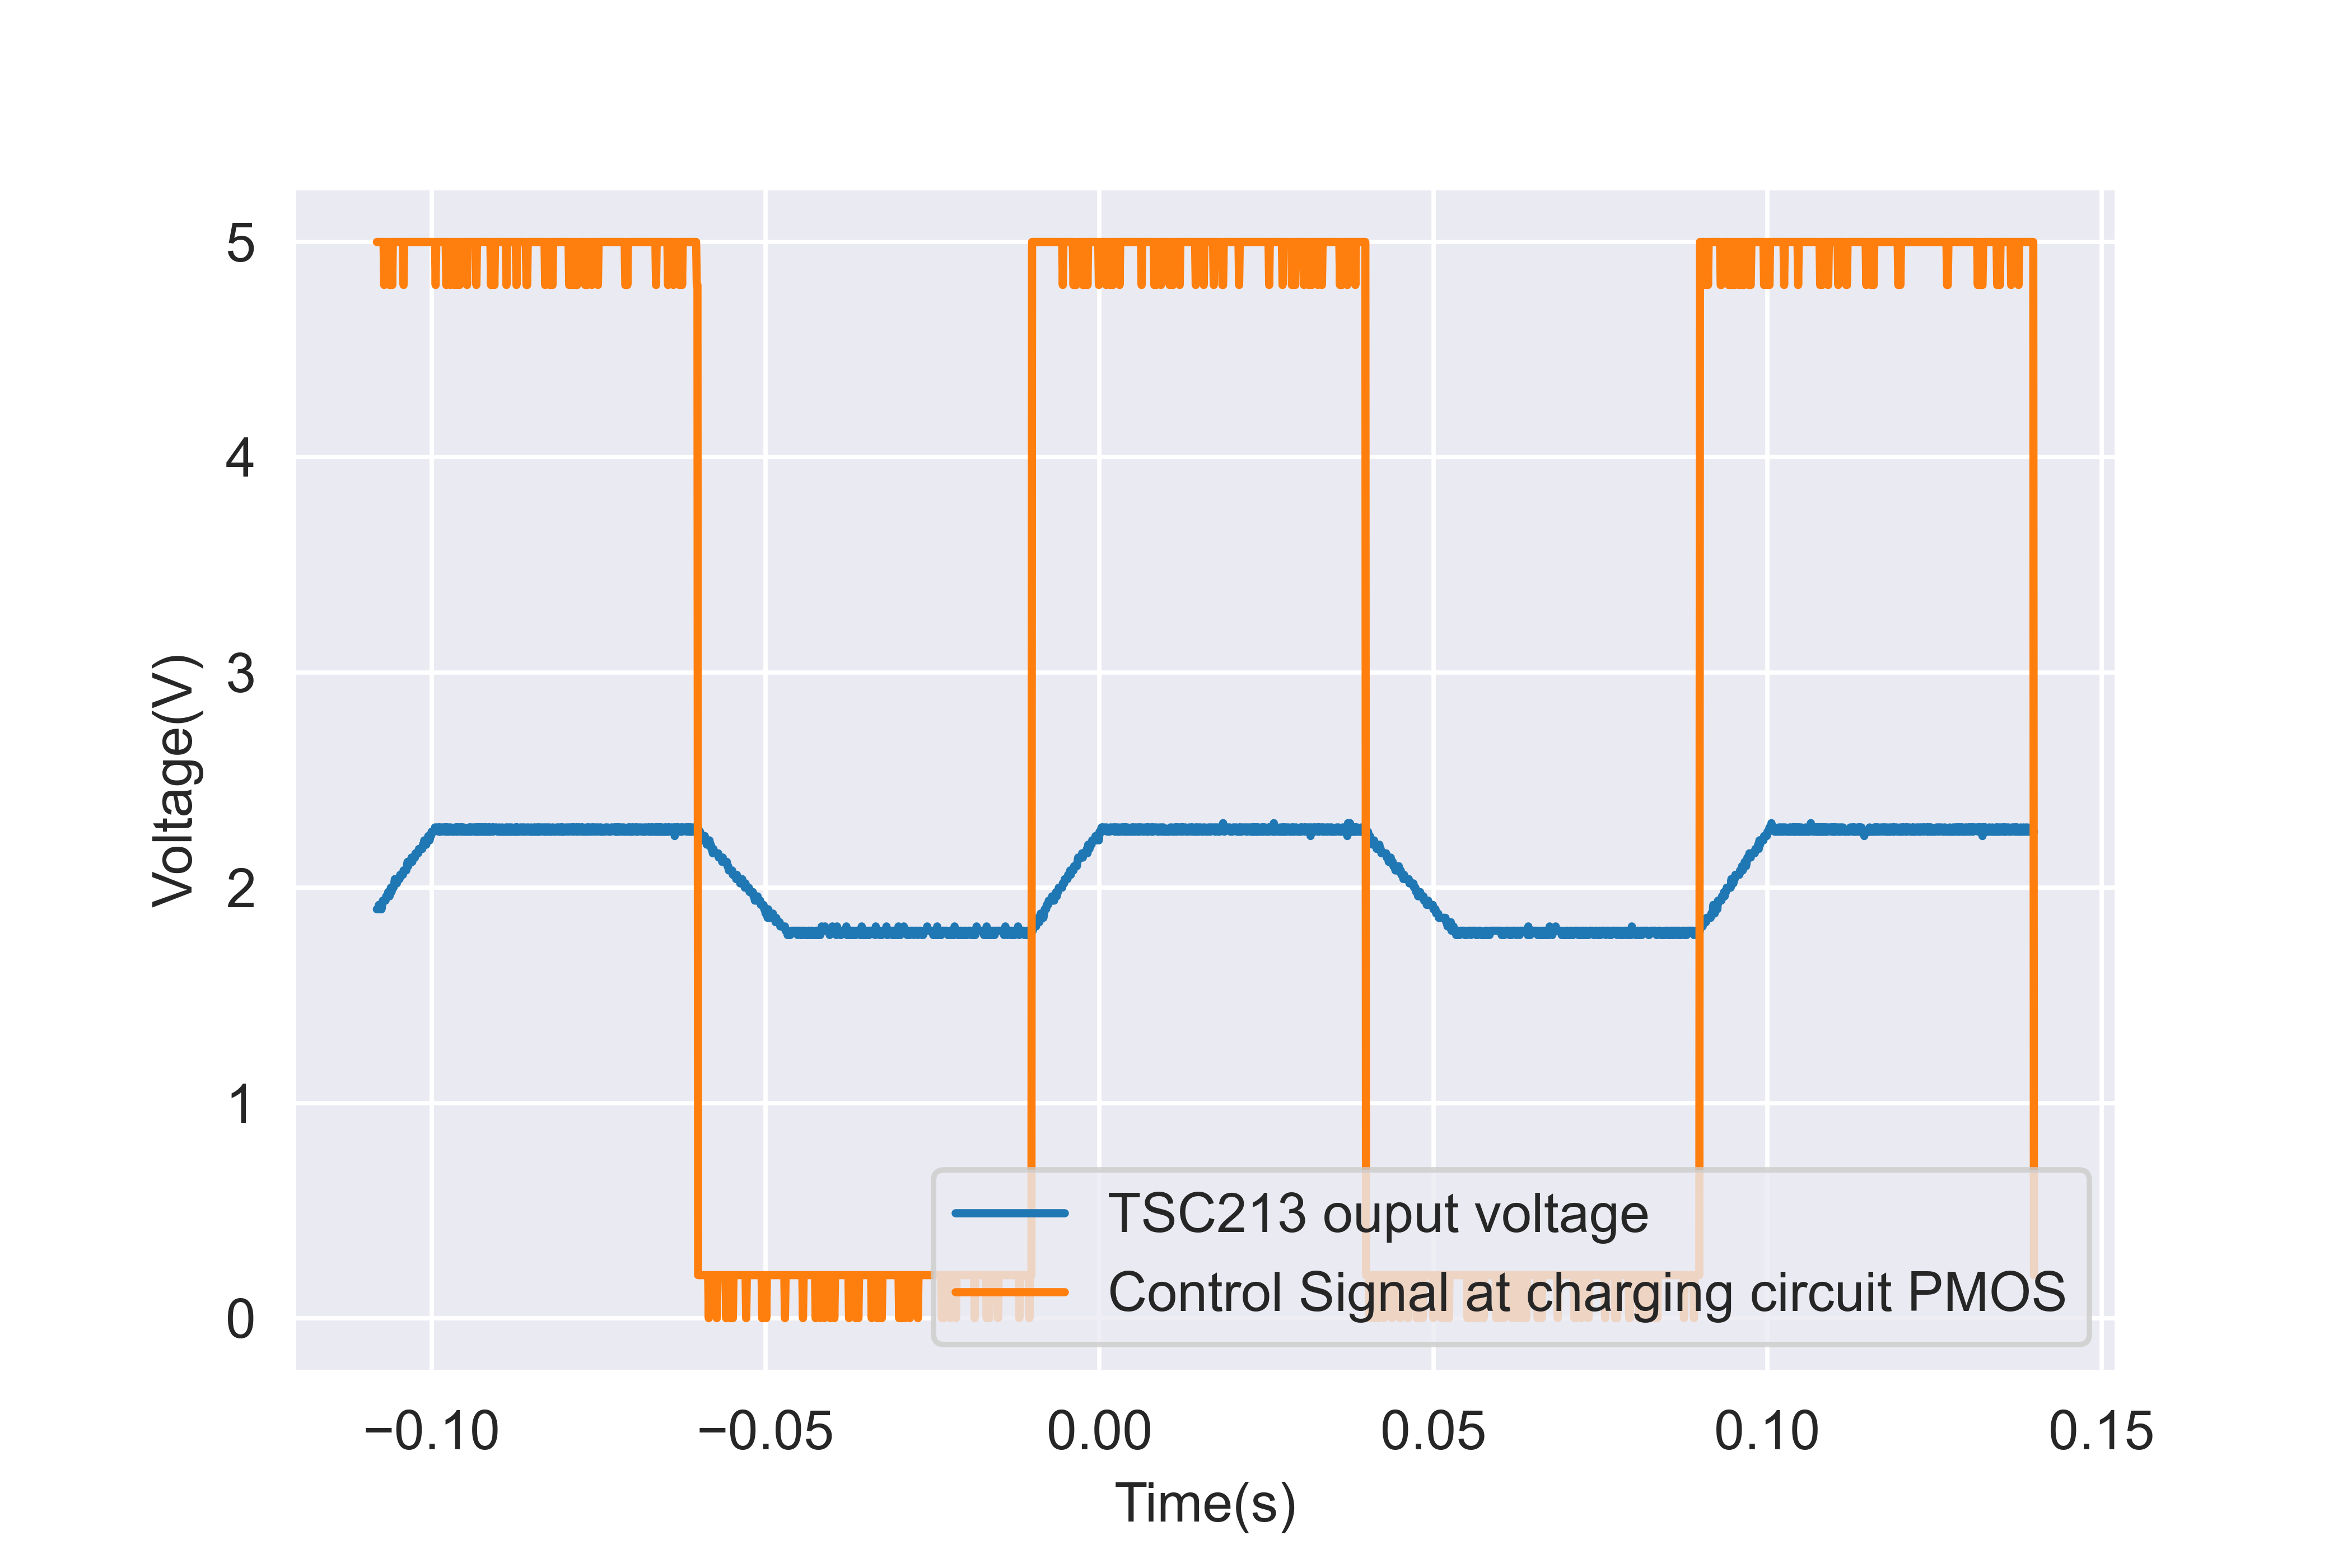
\includegraphics[width=1\linewidth]{./Figures/chargePMOSmeas}
		\caption{} \label{subfig:risePMOS}
	\end{subfigure}
	\begin{subfigure}[]{0.48\textwidth}
		\centering
		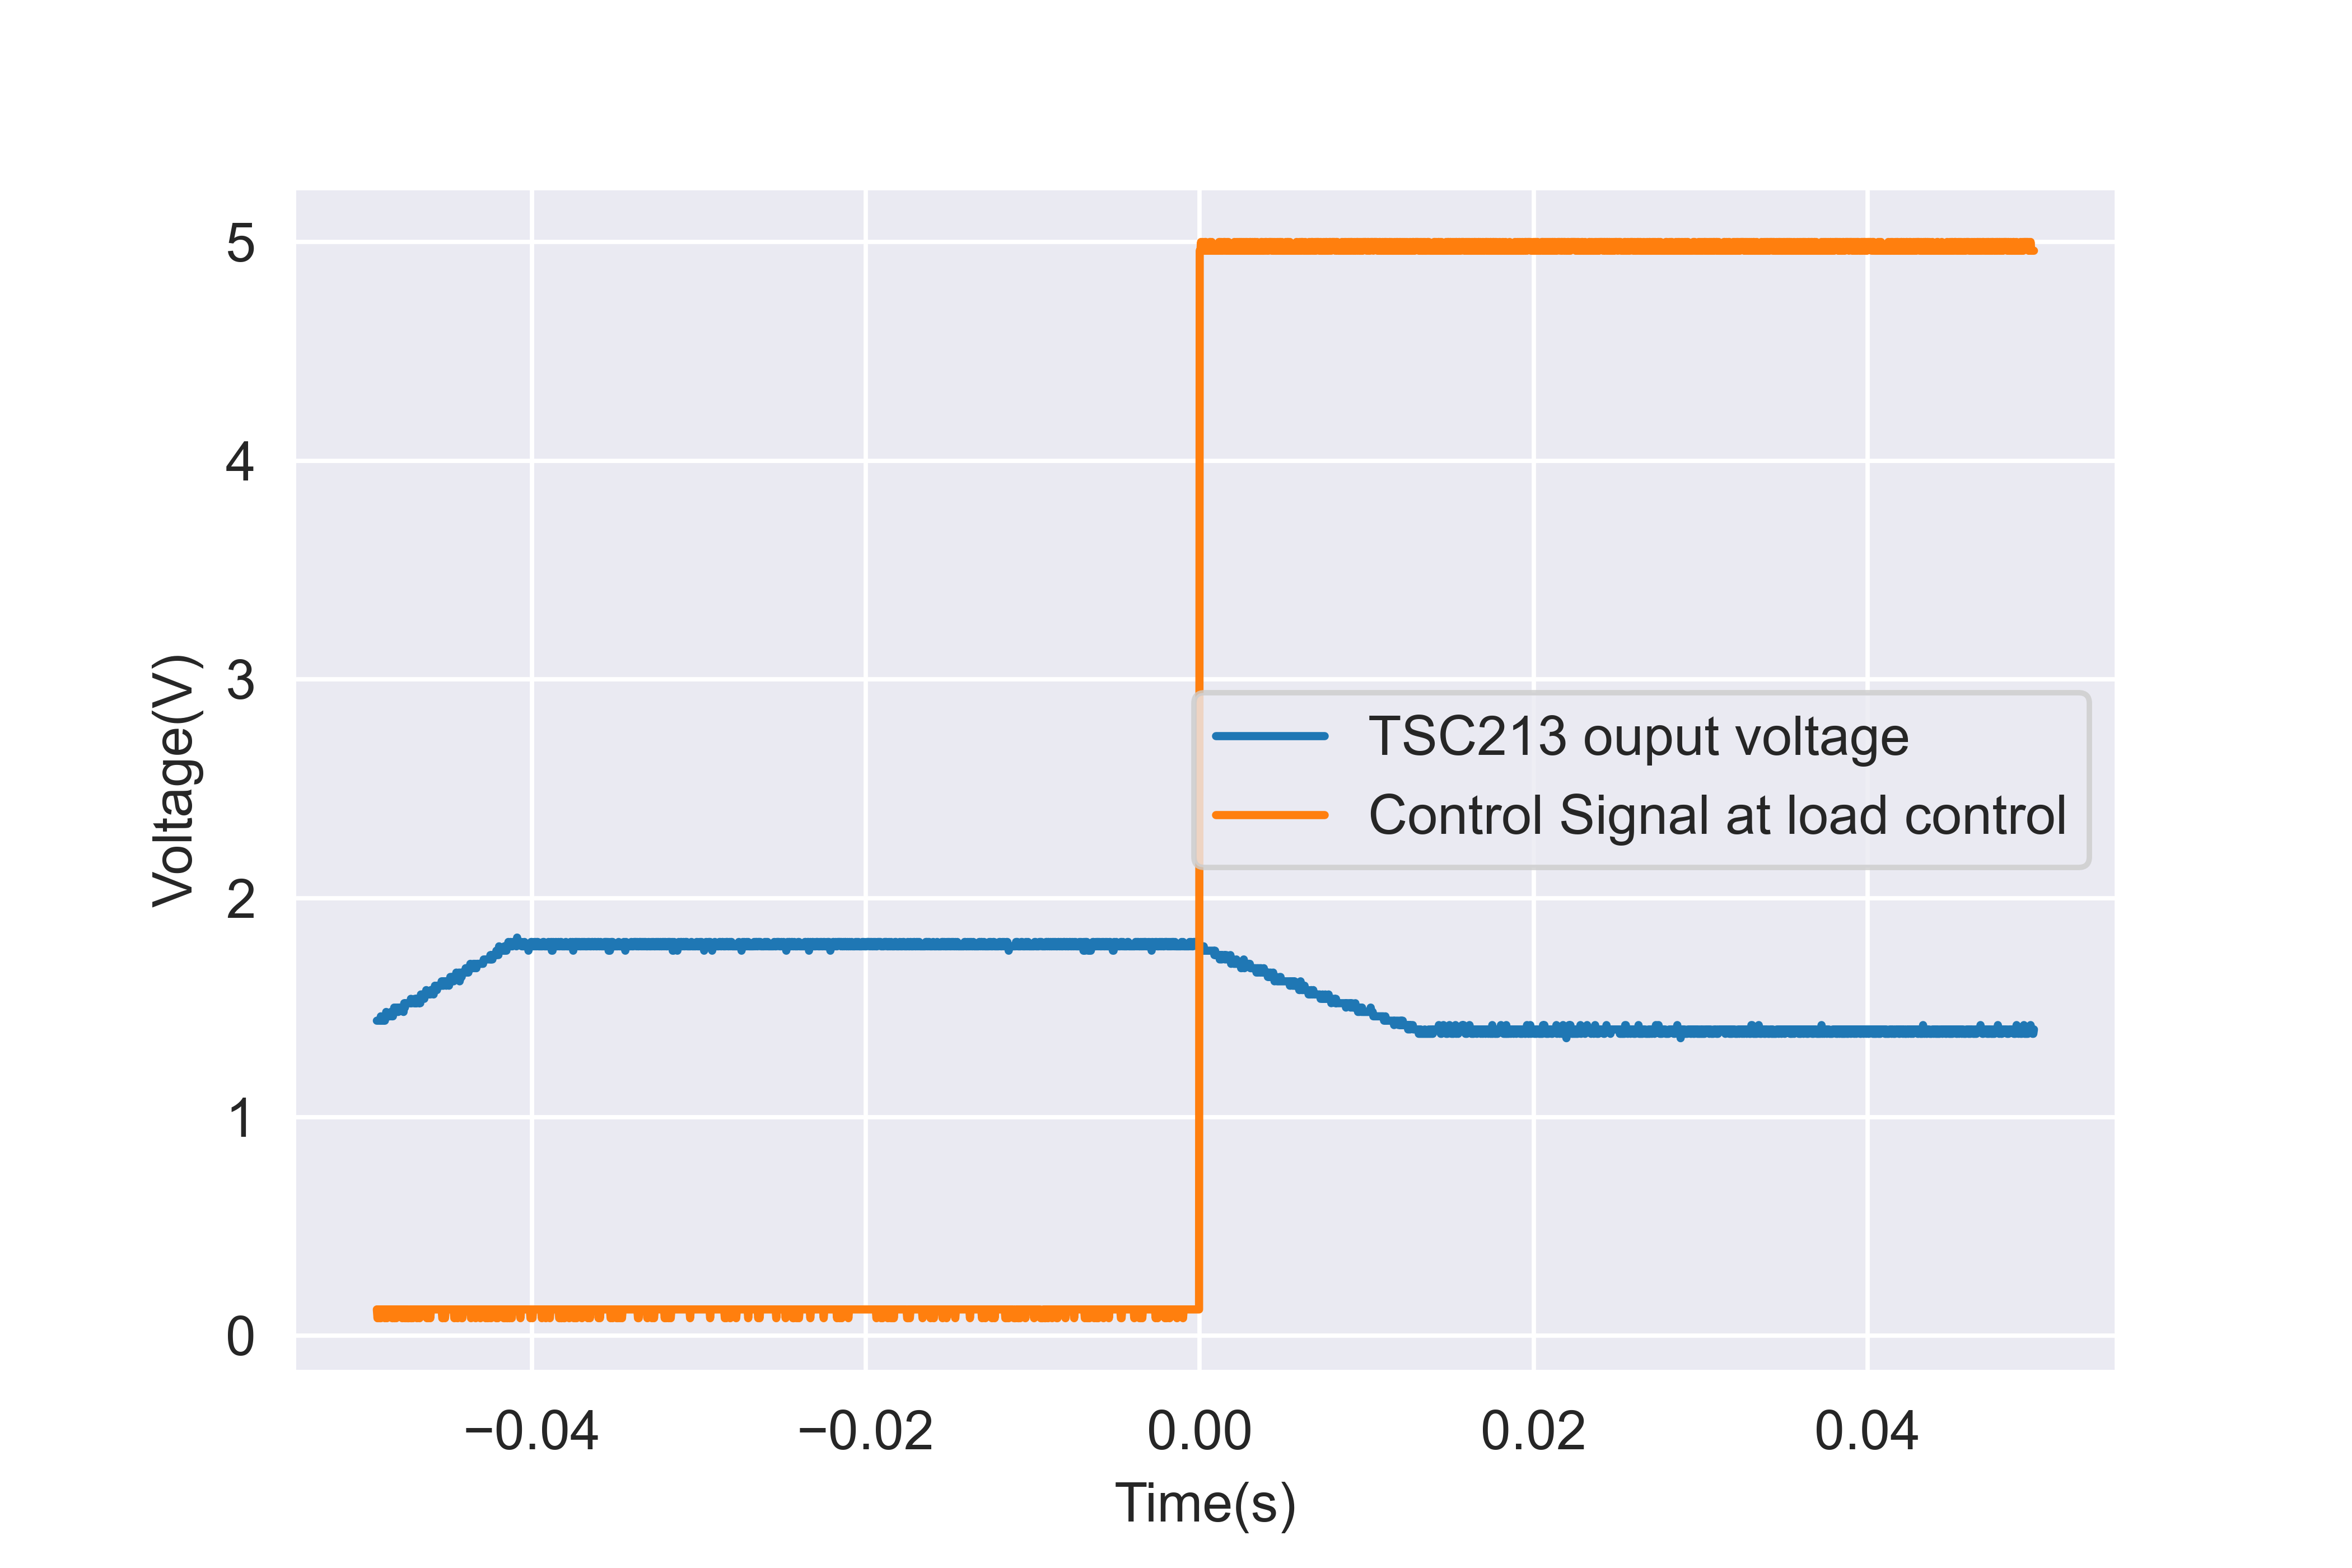
\includegraphics[width=1\linewidth]{./Figures/NMOSTSCmeas}
		\caption{ } \label{subfig:riseNMOS}
	\end{subfigure}
	\caption[{Rise Time for different switches }]{Oscilloscope switch evaluation of in system  (a)  High Side switch used to change TSC output  (b)Low side circuit used to change TSC213 output }
	\label{fig:rise}
\end{figure}

From the 2 figures in figure \ref{fig:rise} it can be said that the switches worked effectively in conjunction with the battery under voltage and charging circuits because as each switched changed state current discharged (NMOS ON, TSC output is below 1.75V) or charged (PMOS ON TSC output is above 1.75V). From these graphs it can also be seen that the time it takes for the output to change is less than 20 milliseconds which is fast.


\begin{figure}[!htb]
	\centering
	\includegraphics[width=0.85\linewidth]{Figures/numx.png}
	\caption{Circuit with barcode and Student Card}
	\label{fig:required}
\end{figure}